\chapter{Hiện thực và Kiểm thử}

\section{Hiện thực hệ thống}
Hệ thống học tập được triển khai nhằm hỗ trợ sinh viên và giảng viên trong việc tổ chức và quản lý việc học tập hiệu quả hơn. Với sự hỗ trợ của Mô hình Ngôn ngữ Lớn (LLMs), hệ thống có thể tự động tạo ra các bài học đề xuất dựa trên mục tiêu học tập của sinh viên và nội dung được cung cấp bởi giảng viên.

Hệ thống được thiết kế với kiến trúc phân tách rõ ràng giữa frontend và backend, sử dụng các công nghệ hiện đại để đảm bảo tính linh hoạt, dễ mở rộng và bảo trì.

\textbf{Frontend} 

Frontend được xây dựng bằng VueJS, tích hợp Vuetify và Tailwind CSS để cung cấp giao diện người dùng trực quan, hiện đại và dễ sử dụng. Các chức năng chính bao gồm:

\begin{itemize}
    \item Quản lý dashboard của sinh viên
    \item Hiển thị danh sách khóa học, chi tiết khóa học
    \item Gửi phản hồi và nhập mục tiêu học tập
\end{itemize}

\begin{figure}[H]
    \centering
    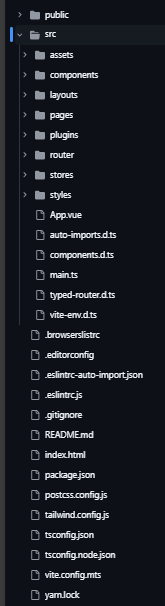
\includegraphics[scale=0.5]{Images/Implement/frontendStructure.png}
    \caption{Cấu trúc Frontend}
\end{figure}

\subsection*{Hệ thống thiết kế (Design System)}

Hệ thống thiết kế được triển khai với mục tiêu cung cấp một giao diện người dùng nhất quán, dễ sử dụng và dễ mở rộng. Hệ thống này bao gồm các thành phần chính sau:

\subsubsection*{Typography}
Typography được xây dựng trên cơ sở font chữ Public Sans, với nhiều kích cỡ và độ đậm khác nhau để phục vụ các nhu cầu hiển thị khác nhau. Font chữ này được chọn vì dễ đọc, phù hợp với các thiết kế hiện đại và hỗ trợ đa ngôn ngữ. Các cấp độ bao gồm:

\begin{itemize}
    \item \textbf{Heading}: Từ Heading 1 (48px, Bold) đến Heading 4 (24px, Semibold).
    \item \textbf{Body Text}: Các cấp độ từ Large đến Small, sử dụng độ đậm từ Regular đến Bold, kích thước từ 10px đến 20px.
\end{itemize}

\begin{figure}[H]
    \centering
    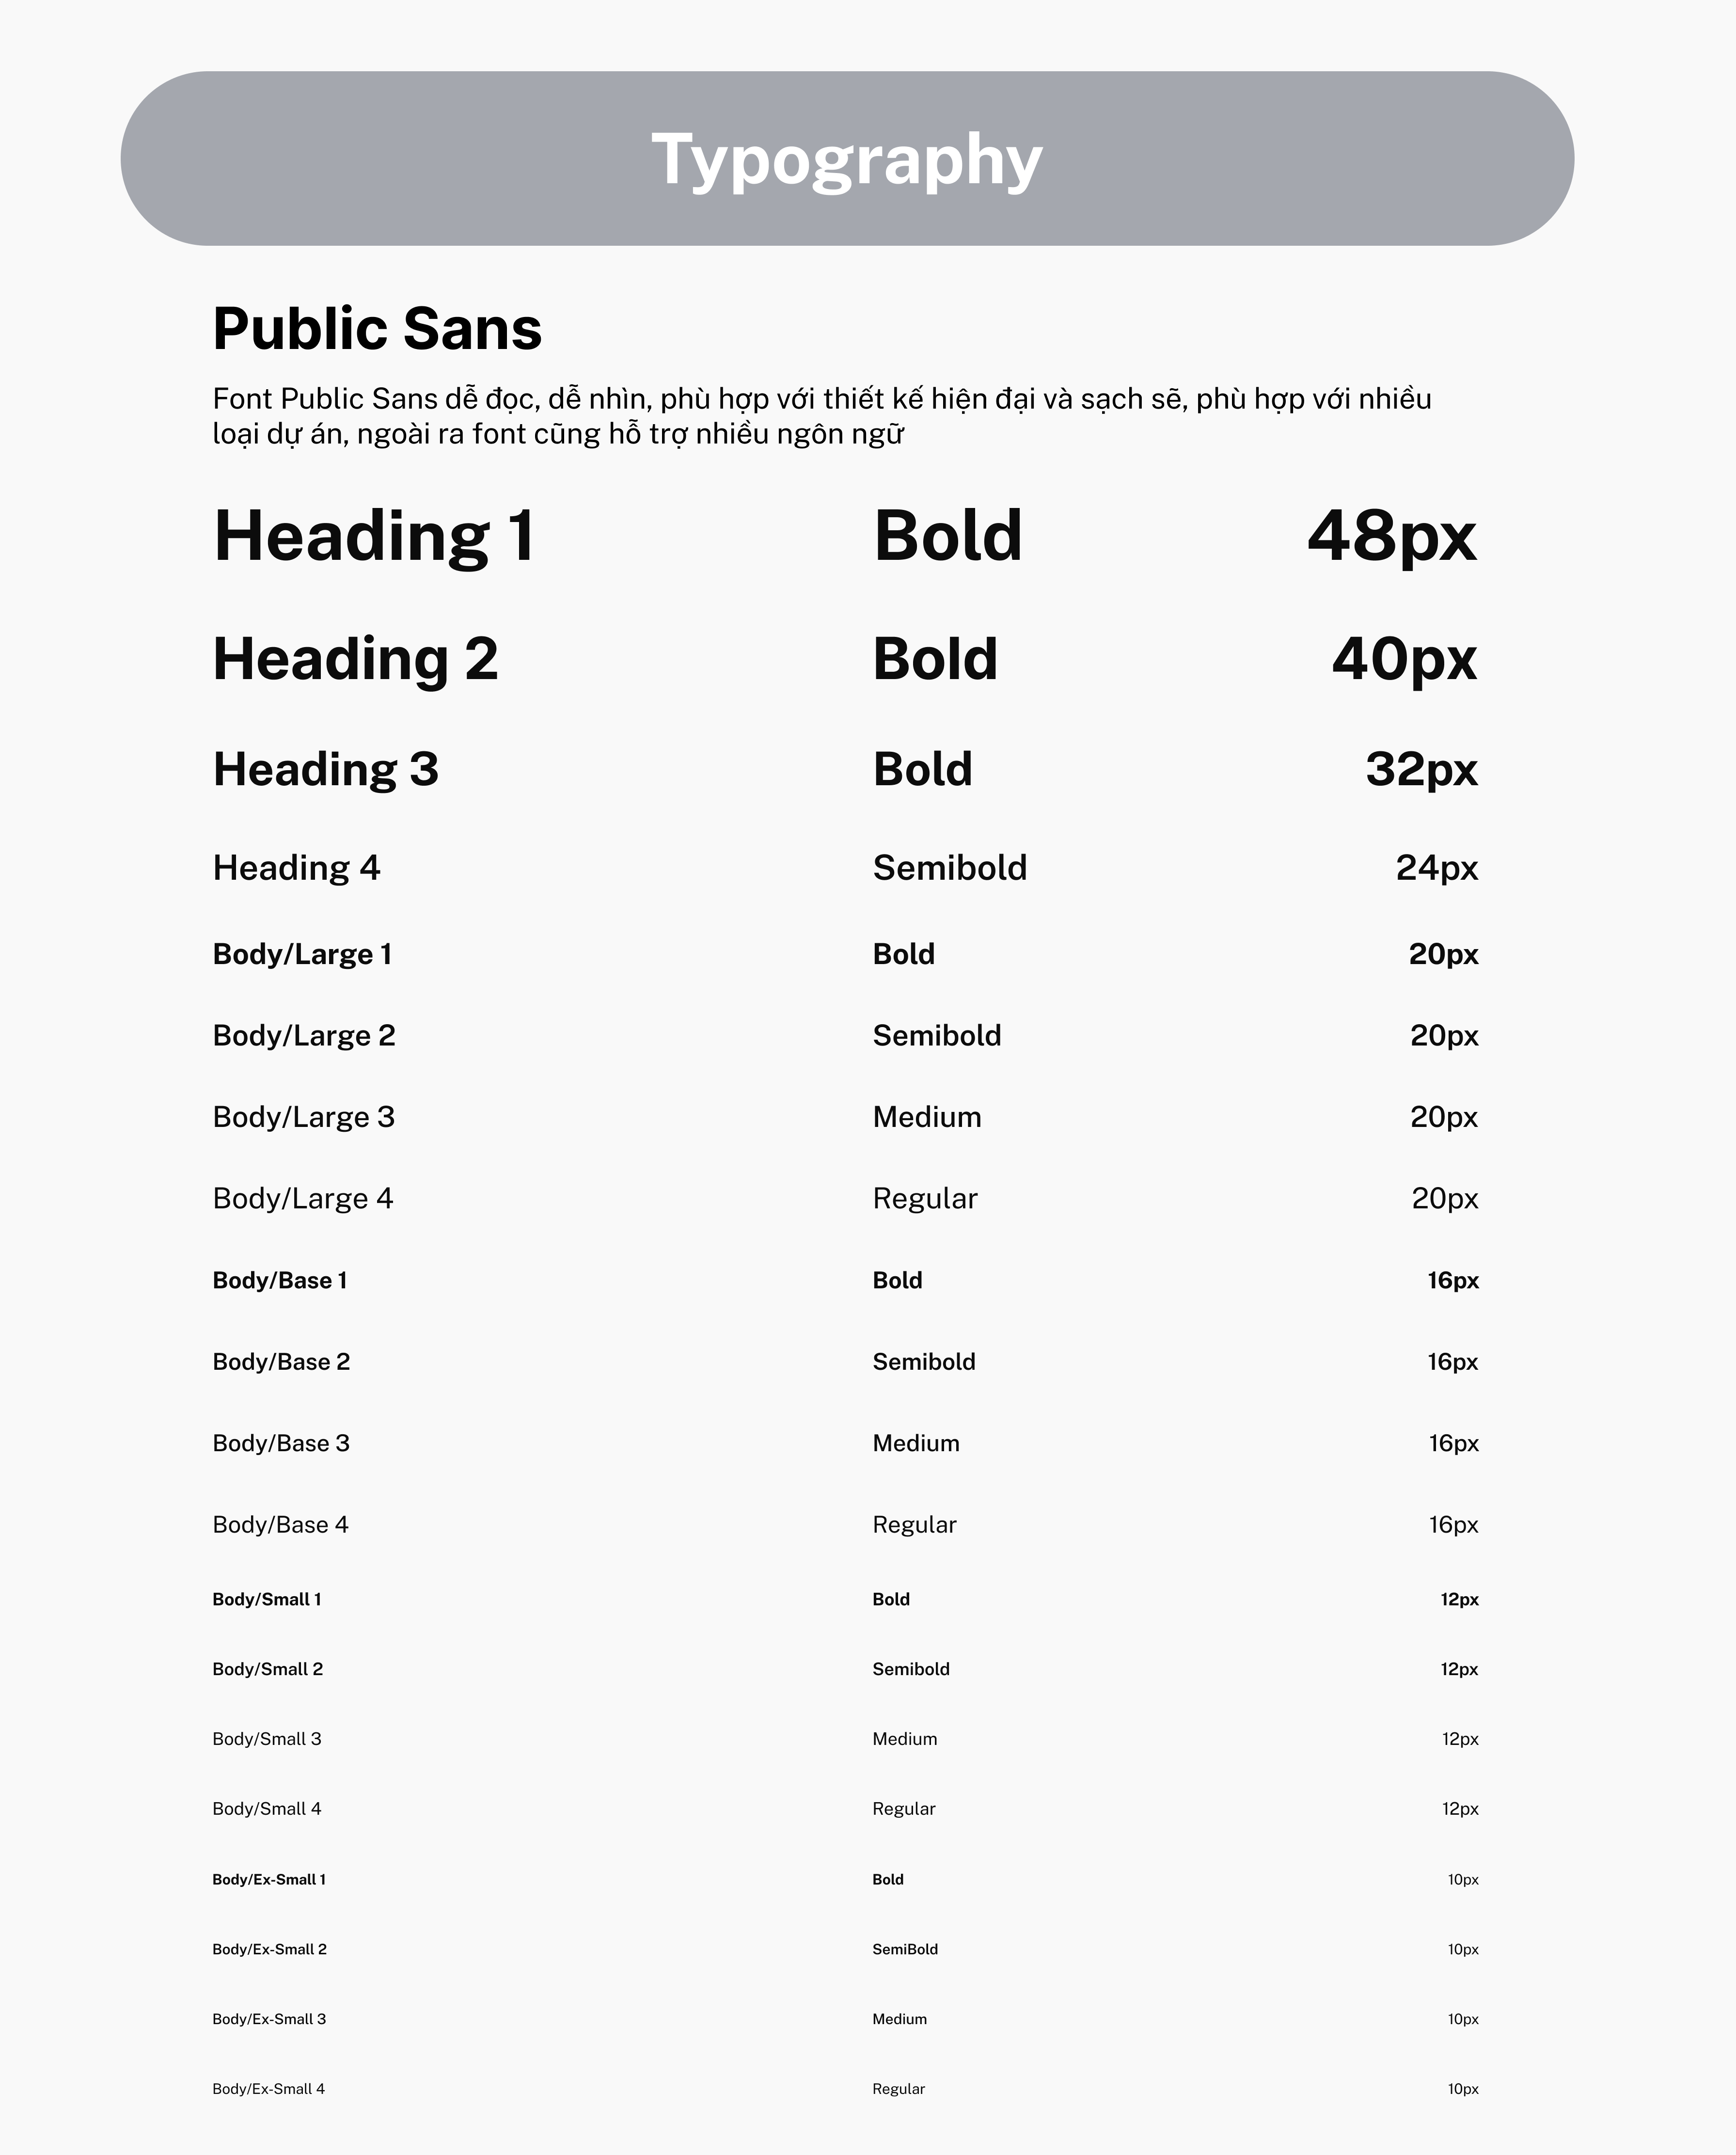
\includegraphics[scale=0.3]{Images/Implement/Typography.png}
    \caption{Hệ thống Typography sử dụng trong ứng dụng}
\end{figure}

\subsubsection*{Bảng màu (Color Palette)}
Bảng màu được thiết kế để mang lại sự nhất quán và dễ nhận biết trong giao diện người dùng. Bảng màu chính bao gồm các màu \textbf{Primary}, \textbf{Secondary}, và các trạng thái như \textbf{Error}, \textbf{Warning}, \textbf{Neutral}, \textbf{Success}. Mỗi màu được chia thành các sắc độ từ nhạt (25, 50) đến đậm (900, 950), nhằm đảm bảo khả năng hiển thị tốt trong các trường hợp sử dụng khác nhau.

\begin{itemize}
    \item \textbf{Primary}: Dùng cho các thành phần chính như nút bấm và tiêu đề.
    \item \textbf{Secondary}: Dùng cho các chi tiết phụ hoặc nhấn mạnh nội dung.
    \item \textbf{Error, Warning, Success}: Dùng để phản hồi trạng thái của hệ thống.
\end{itemize}

\begin{figure}[H]
    \centering
    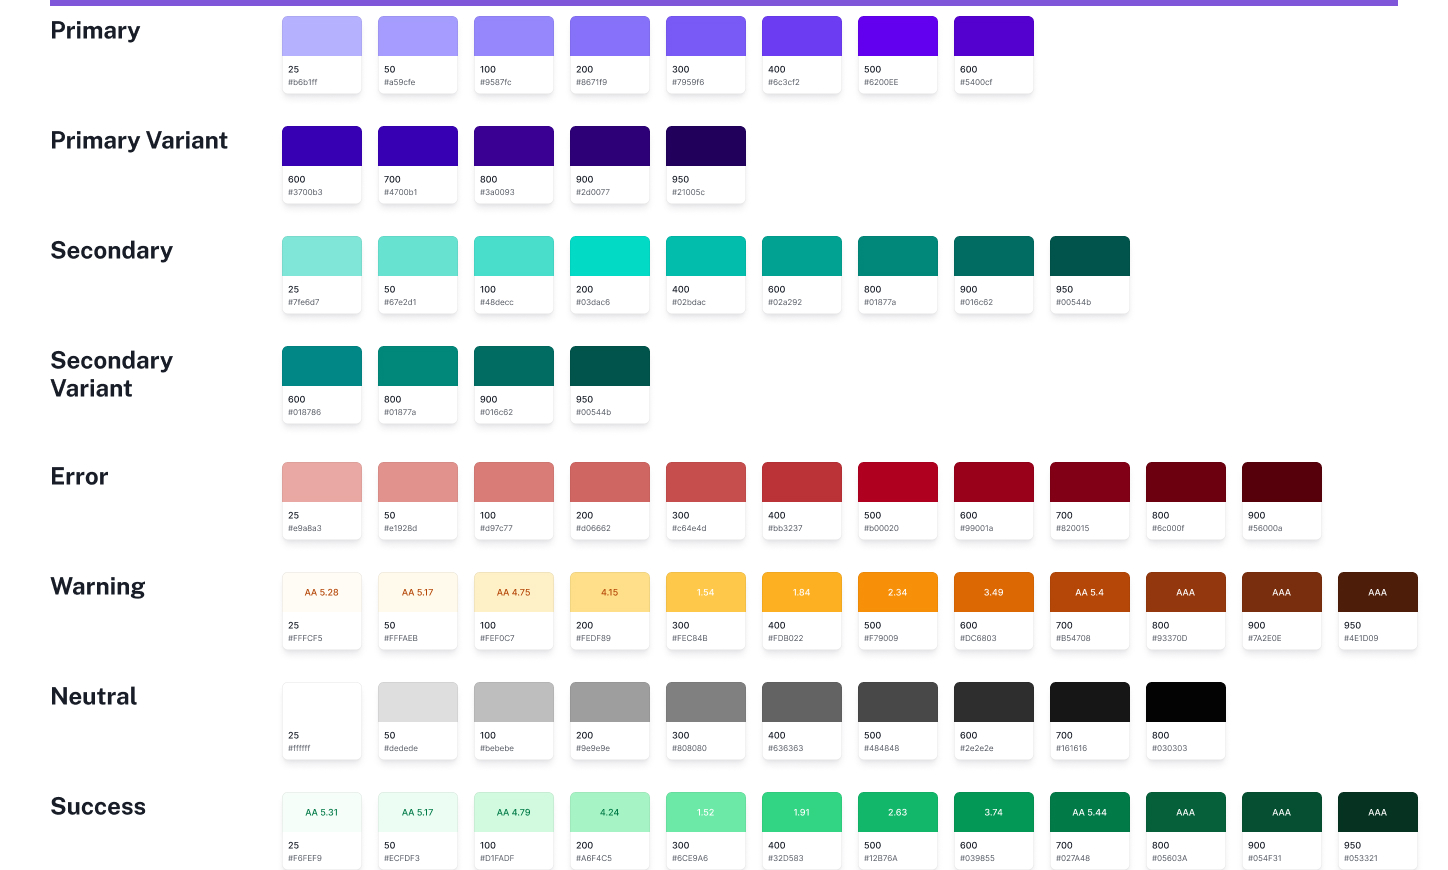
\includegraphics[scale=0.15]{Images/Implement/Colors.jpg}
    \caption{Bảng màu được sử dụng trong ứng dụng}
\end{figure}

Hệ thống này được tích hợp với Tailwind CSS, giúp tự động hóa việc áp dụng các quy tắc thiết kế (design tokens) vào mã nguồn. Điều này làm giảm thiểu lỗi thiết kế, đồng thời đảm bảo giao diện nhất quán trong toàn bộ ứng dụng.


\textbf{Backend}

Backend được phát triển với FastAPI, kết hợp với PostgreSQL để lưu trữ dữ liệu. Kiến trúc hệ thống được tổ chức theo các thành phần chính:

\begin{itemize}
    \item Repository
    \item Provider
    \item Controller
\end{itemize}

Mỗi thành phần đảm nhiệm một vai trò cụ thể, giúp hệ thống trở nên dễ hiểu, có tính tổ chức cao và dễ bảo trì.

\begin{figure}[H]
    \centering
    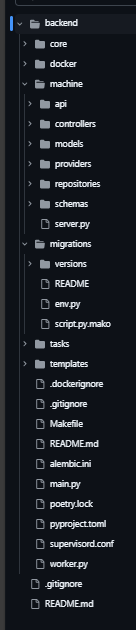
\includegraphics[scale=0.5]{Images/Implement/backendStructure.png}
    \caption{Cấu trúc Backend}
\end{figure}

\section{Kiến trúc Backend}

\textbf{1. Repository} 

Repository chịu trách nhiệm quản lý các thao tác liên quan đến dữ liệu trong hệ thống. Đây là nơi thực hiện các logic liên quan đến việc truy vấn, lưu trữ và cập nhật dữ liệu từ cơ sở dữ liệu PostgreSQL.

Đặc điểm chính:

\begin{itemize}
    \item Tách biệt logic truy xuất dữ liệu khỏi các thành phần khác
    \item Hỗ trợ các thao tác CRUD (Create, Read, Update, Delete)
\end{itemize}

Ví dụ: Repository sẽ xử lý các tác vụ như:

\begin{itemize}
    \item Truy vấn thông tin sinh viên và giảng viên
    \item Cập nhật tiến độ học tập
    \item Xóa thông tin khóa học khi cần thiết
\end{itemize}

\textbf{2. Provider} 

Provider chịu trách nhiệm xử lý các logic nghiệp vụ (business logic). Đây là nơi các phép toán và xử lý phức tạp được thực hiện trước khi trả kết quả cho Controller hoặc người dùng.

Đặc điểm chính:

\begin{itemize}
    \item Không phụ thuộc vào giao diện hoặc nguồn dữ liệu cụ thể
    \item Tập trung vào logic nghiệp vụ và các phép toán quan trọng
\end{itemize}

Ví dụ: Provider sẽ:

\begin{itemize}
    \item Phân tích mục tiêu học tập của sinh viên để đề xuất bài học
    \item Tự động tạo bài học dựa trên nội dung được giảng viên cung cấp
\end{itemize}
 
\textbf{3. Controller} 

Controller là nơi tiếp nhận các yêu cầu từ người dùng thông qua API, sau đó phối hợp với Provider và Repository để thực hiện các chức năng tương ứng.

Đặc điểm chính:

\begin{itemize}
    \item Giao tiếp trực tiếp với frontend thông qua các endpoint API
    \item Chuyển đổi dữ liệu giữa frontend và các thành phần backend
\end{itemize}

Ví dụ: Controller xử lý:

\begin{itemize}
    \item Yêu cầu đăng nhập và xác thực người dùng
    \item Truy xuất danh sách khóa học và chi tiết khóa học
    \item Nhận mục tiêu học tập từ sinh viên và gửi đến Provider để xử lý
\end{itemize}

\section{Quá trình triển khai hệ thống}

\textbf{1. Tạo cấu trúc cơ sở dữ liệu} 

Cơ sở dữ liệu được thiết kế để lưu trữ các thông tin liên quan đến sinh viên, giảng viên, khóa học và bài học. Sơ đồ dưới đây minh họa cấu trúc cơ sở dữ liệu:

\begin{figure}[H]
    \centering
    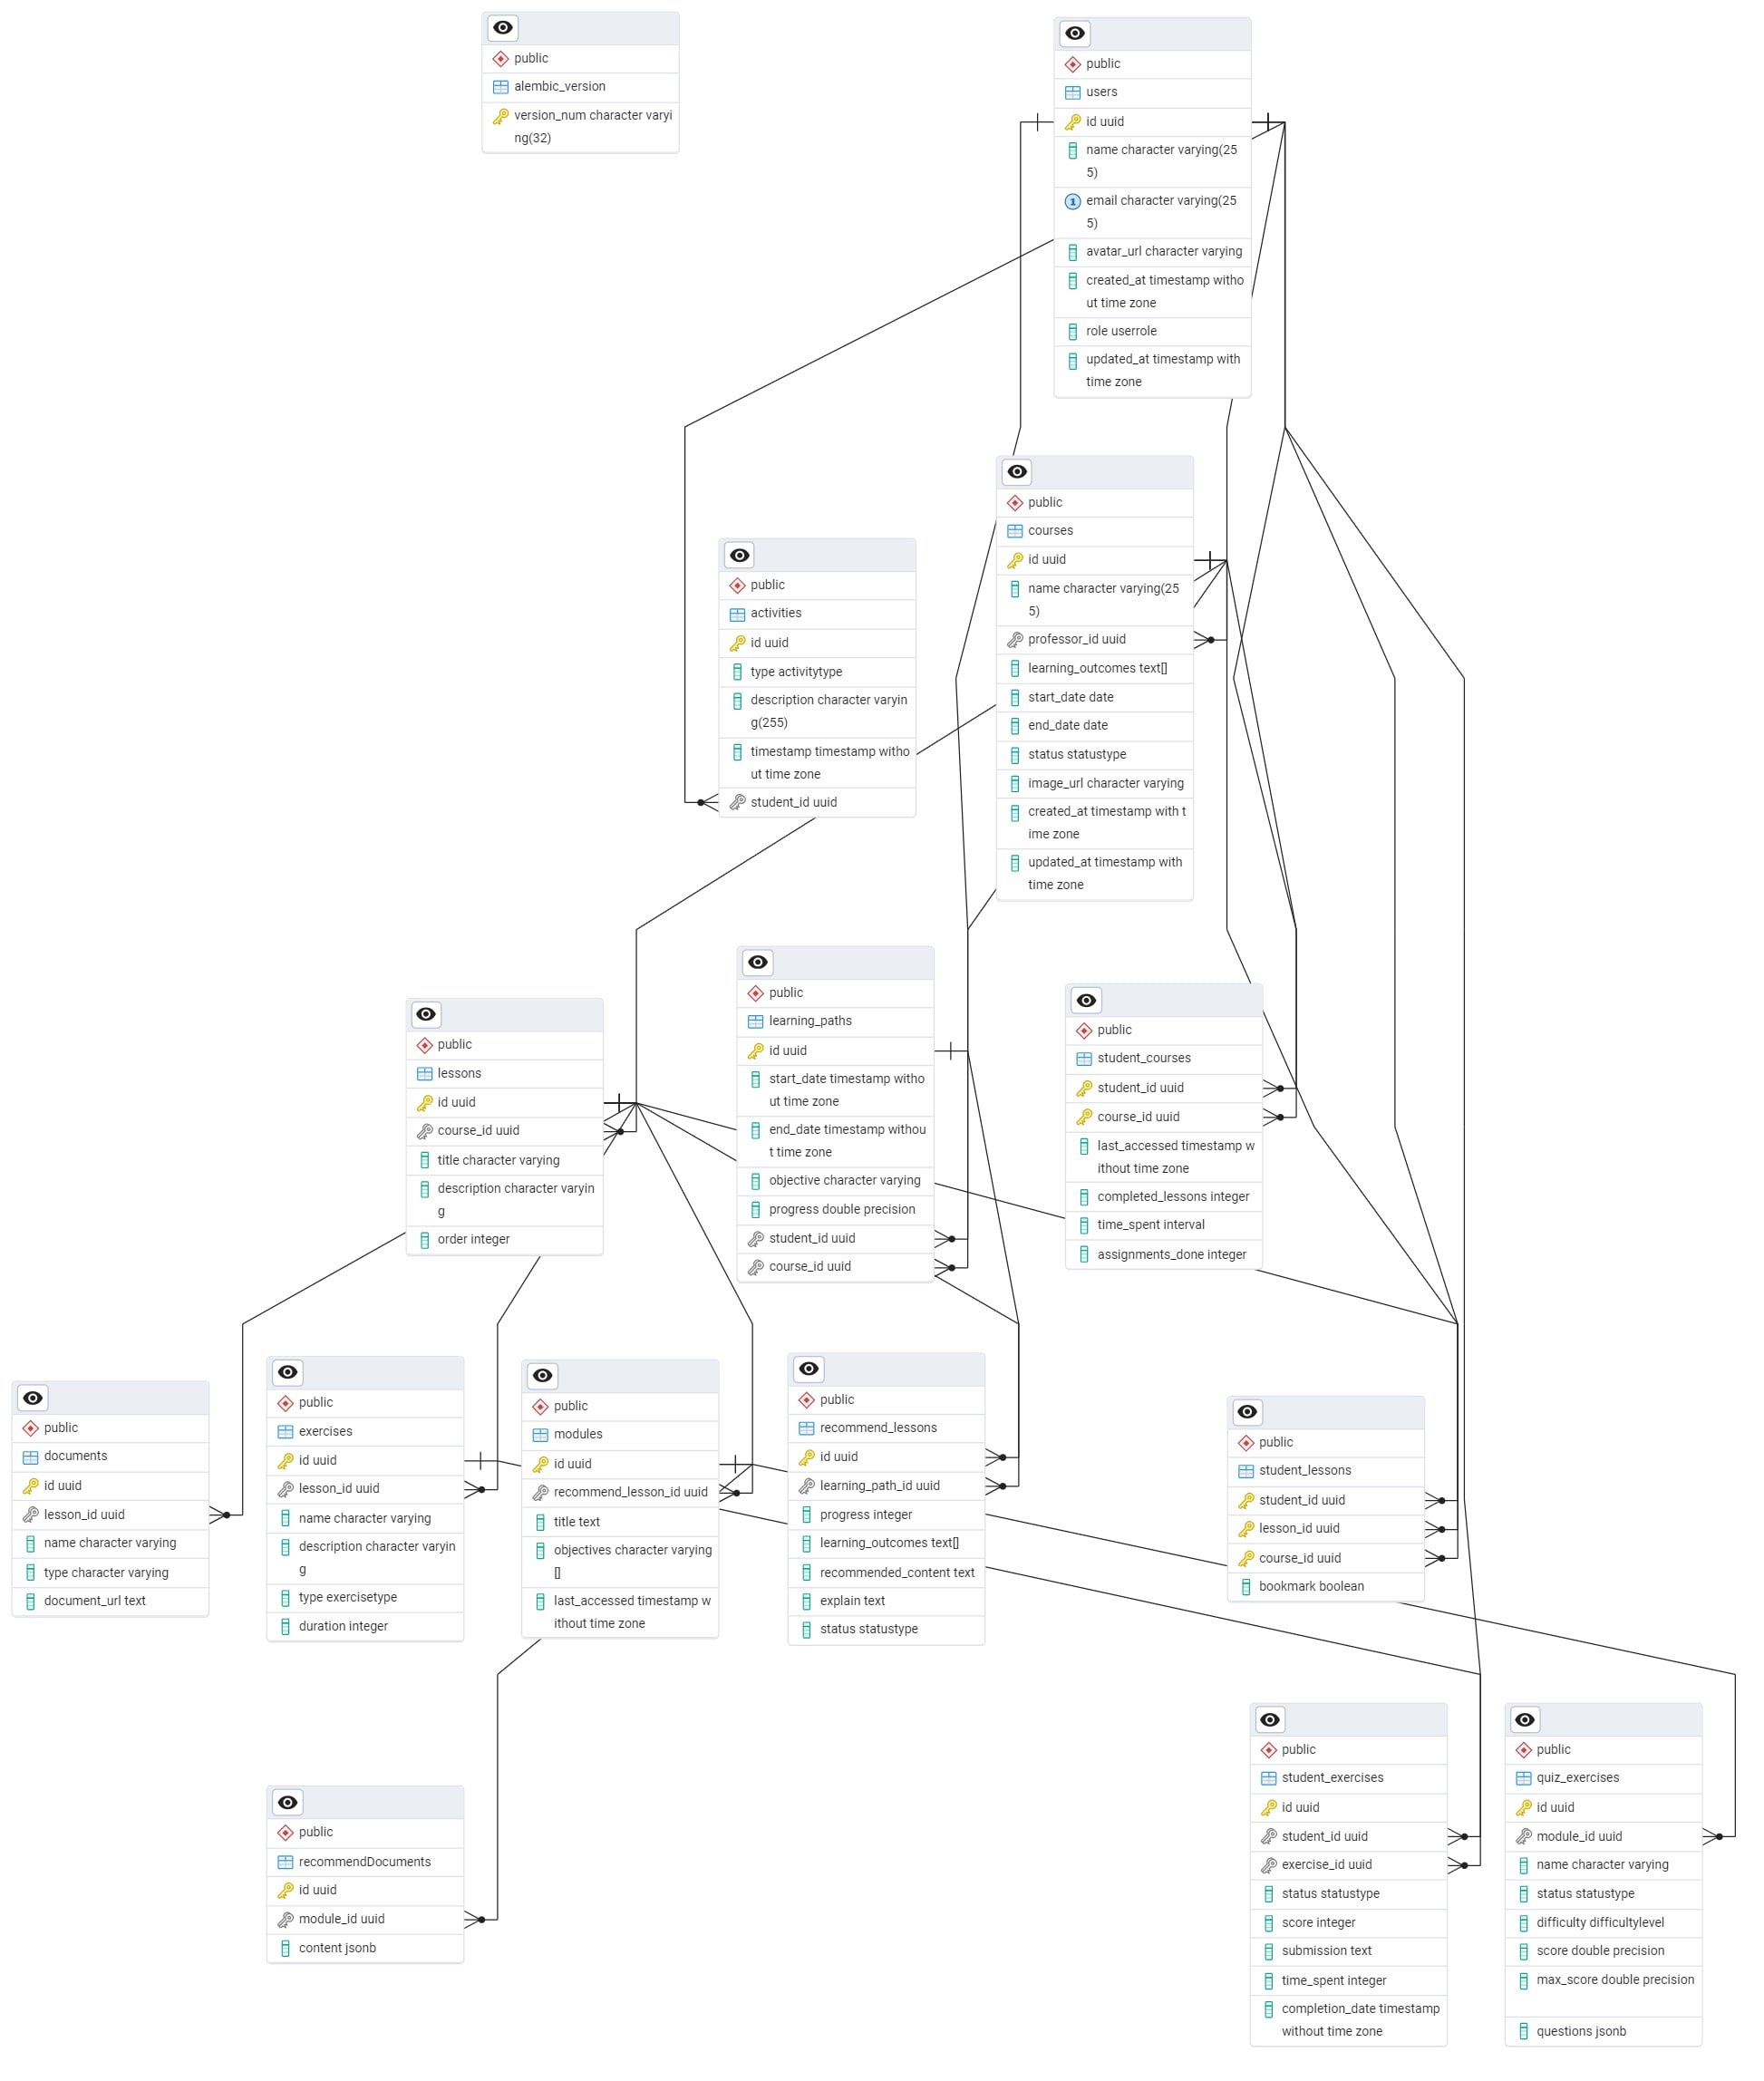
\includegraphics[width=0.8\textwidth]{Images/Implement/DB_diagram.jpg}
    \caption{Cấu trúc Cơ sở dữ liệu}
\end{figure}

\textbf{2. Xây dựng API} 

Các API hỗ trợ giao tiếp giữa frontend và backend, đảm bảo rằng người dùng có thể tương tác với hệ thống một cách hiệu quả. Các chức năng chính của API bao gồm:

\begin{itemize}
    \item Quản lý khóa học
    \item Quản lý bài học
    \item Gửi và nhận phản hồi từ sinh viên
\end{itemize}

FastAPI cung cấp cơ chế xử lý yêu cầu nhanh chóng và an toàn, giúp cải thiện hiệu năng hệ thống.

\textbf{3. Quản lý bài học và đề xuất học tập} 

Hệ thống sử dụng LLMs để phân tích dữ liệu từ sinh viên và giảng viên, từ đó đưa ra các bài học phù hợp. Điều này giúp cá nhân hóa việc học tập và tăng hiệu quả của hệ thống.

Cụ thể:

\begin{itemize}
    \item Giảng viên cung cấp nội dung khóa học và mục tiêu học
    \item Sinh viên nhập mục tiêu học tập cá nhân
    \item LLMs xử lý và đề xuất các bài học tương thích
\end{itemize}

\textbf{4. Triển khai hệ thống}

\textbf{Frontend:}
Frontend của hệ thống được triển khai trên nền tảng \textbf{Vercel}, mang đến một môi trường ổn định, tối ưu cho việc triển khai các ứng dụng web. Vercel cung cấp khả năng tự động build và deploy mỗi khi có thay đổi trong mã nguồn, giúp quá trình cập nhật trở nên nhanh chóng và mượt mà. Nhờ vào quy trình này, việc triển khai và duy trì hệ thống frontend trở nên đơn giản và hiệu quả.

Vercel không chỉ đảm bảo hiệu suất cao mà còn hỗ trợ các tính năng tối ưu hóa tự động, giúp giảm thời gian tải trang và nâng cao trải nghiệm người dùng. Với khả năng mở rộng linh hoạt, hệ thống có thể dễ dàng đáp ứng với nhu cầu tăng trưởng trong tương lai.

\par \textbf{Link deploy frontend:} \textcolor{blue}{\href{https://codemate-fe-murex.vercel.app/}{https://codemate-fe-murex.vercel.app/}}

\textbf{Backend:}
Hệ thống sử dụng nền tảng \textbf{Render} để triển khai backend. Render cung cấp một môi trường chạy ổn định, dễ mở rộng và bảo mật cao, giúp tối ưu hóa việc quản lý và triển khai ứng dụng. Với quy trình build và deploy tự động, việc cập nhật hệ thống trở nên mượt mà và hiệu quả, giảm thiểu các vấn đề phát sinh trong quá trình triển khai.

Để triển khai hệ thống, chúng tôi sử dụng công cụ \textbf{Poetry} để quản lý các gói phụ thuộc (dependencies) của Python. Điều này giúp đảm bảo rằng các thư viện và công cụ cần thiết luôn được cài đặt đúng phiên bản, đồng thời giảm thiểu các lỗi liên quan đến môi trường chạy.

Hệ thống được cấu hình để tự động khởi chạy khi có yêu cầu, đảm bảo hiệu suất cao và khả năng mở rộng dễ dàng khi cần thiết. Ngoài ra, Render cũng hỗ trợ giám sát và quản lý môi trường ứng dụng, giúp dễ dàng phát hiện và xử lý các sự cố.

\par \textbf{Link deploy backend:} \textcolor{blue}{\href{https://edumind.onrender.com}{https://edumind.onrender.com}}



\section{Kiểm thử}

\subsection{Tổng quan về kiểm thử}

Mục đích của kiểm thử trong hệ thống: Đảm bảo rằng các tính năng hoạt động đúng, hệ thống không có lỗi và có thể chịu được tải trong quá trình sử dụng thực tế.

\subsubsection{Loại kiểm thử thực hiện}
\begin{itemize}
    \item \textbf{Kiểm thử chức năng:} Đảm bảo các chức năng của hệ thống hoạt động đúng
    \item \textbf{Kiểm thử hiệu suất:} Đảm bảo hệ thống có thể xử lý nhiều yêu cầu đồng thời
    \item \textbf{Kiểm thử bảo mật:} Đảm bảo hệ thống bảo vệ tốt các dữ liệu người dùng
    \item \textbf{Kiểm thử tích hợp:} Kiểm tra sự hoạt động đồng bộ của các module
    \item \textbf{Kiểm thử hồi quy:} Đảm bảo những thay đổi mới không làm hỏng các tính năng cũ
\end{itemize}

\subsection{Kiểm thử API}

\subsection{Mô tả chung về các kịch bản kiểm thử}

Mỗi kịch bản kiểm thử được tổ chức và theo dõi theo bảng sau đây. Các mục chính trong mỗi kịch bản kiểm thử bao gồm:
\begin{itemize}
    \item \textbf{TEST SCENARIO:} Tên kịch bản kiểm thử
    \item \textbf{Screen name/Function name:} Tên màn hình hoặc tên chức năng cần kiểm thử
    \item \textbf{Test case code:} Mã số của test case
    \item \textbf{Number of passed test cases (P):} Số lượng test case đã thành công
    \item \textbf{Number of failed test cases (F):} Số lượng test case không thành công
    \item \textbf{Number of test cases under pending (PE):} Số lượng test case đang chờ xử lý
    \item \textbf{Number of unexecuted test cases:} Số lượng test case chưa được thực hiện
    \item \textbf{Total number of test cases:} Tổng số test case cần kiểm thử
\end{itemize}

\subsubsection{Cấu trúc của một kịch bản kiểm thử}

\begin{itemize}
    \item \textbf{Test case code:} Mã của test case, giúp phân biệt các test case khác nhau
    \item \textbf{Testing Purpose:} Mục đích của việc kiểm thử
    \item \textbf{Steps:} Các bước thực hiện kiểm thử
    \item \textbf{Expected outcome:} Kết quả mong đợi sau khi thực hiện các bước kiểm thử
    \item \textbf{Browser compatibility testing:} Kiểm tra tính tương thích với các trình duyệt phổ biến
    \item \textbf{Test status report:} Báo cáo tình trạng của các lần kiểm thử
\end{itemize}

\subsubsection{Ví dụ về một kịch bản kiểm thử trong bảng Excel}
\begin{figure}[H]
    \centering
    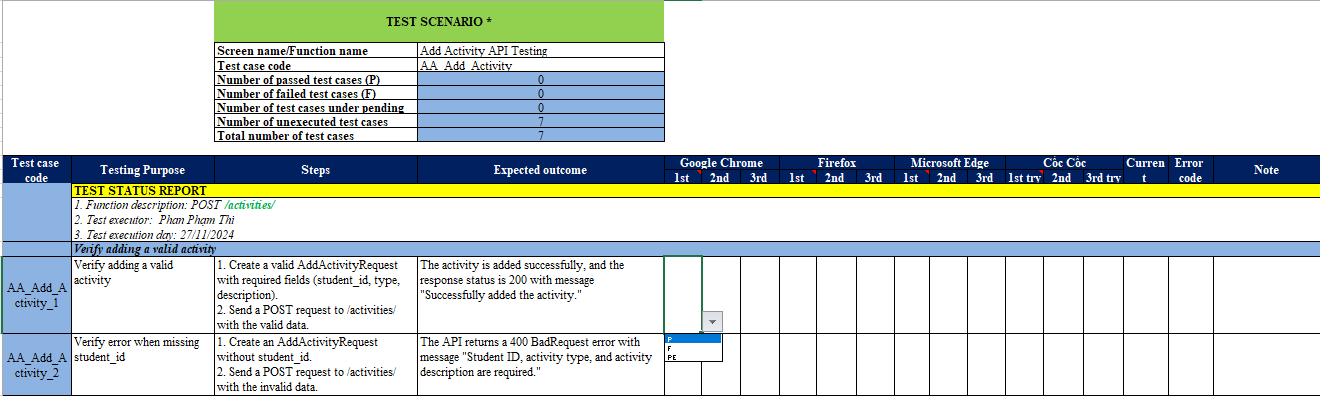
\includegraphics[scale=0.5]{Images/Implement/testScenario.png}
    \caption{Ví dụ về một kịch bản kiểm thử}
\end{figure}
\subsubsection{Mục tiêu của các kịch bản kiểm thử}
\begin{itemize}
    \item \textbf{Kiểm thử chức năng}: Đảm bảo các API hoạt động đúng với các yêu cầu và dữ liệu đầu vào hợp lệ hoặc không hợp lệ. 
    \item \textbf{Kiểm thử tương thích trình duyệt}: Đảm bảo hệ thống hoạt động ổn định trên các trình duyệt phổ biến.
    \item \textbf{Kiểm thử độ tin cậy}: Kiểm tra xem các API có thể xử lý được các tình huống thực tế và đưa ra kết quả chính xác.
\end{itemize}
\subsubsection{Kết quả kiểm thử API}
\subsubsubsection{Kiểm thử phương thức}
\begin{itemize}
    \item \textbf{Welcome API Testing}
    \begin{figure}[H]
        \centering
        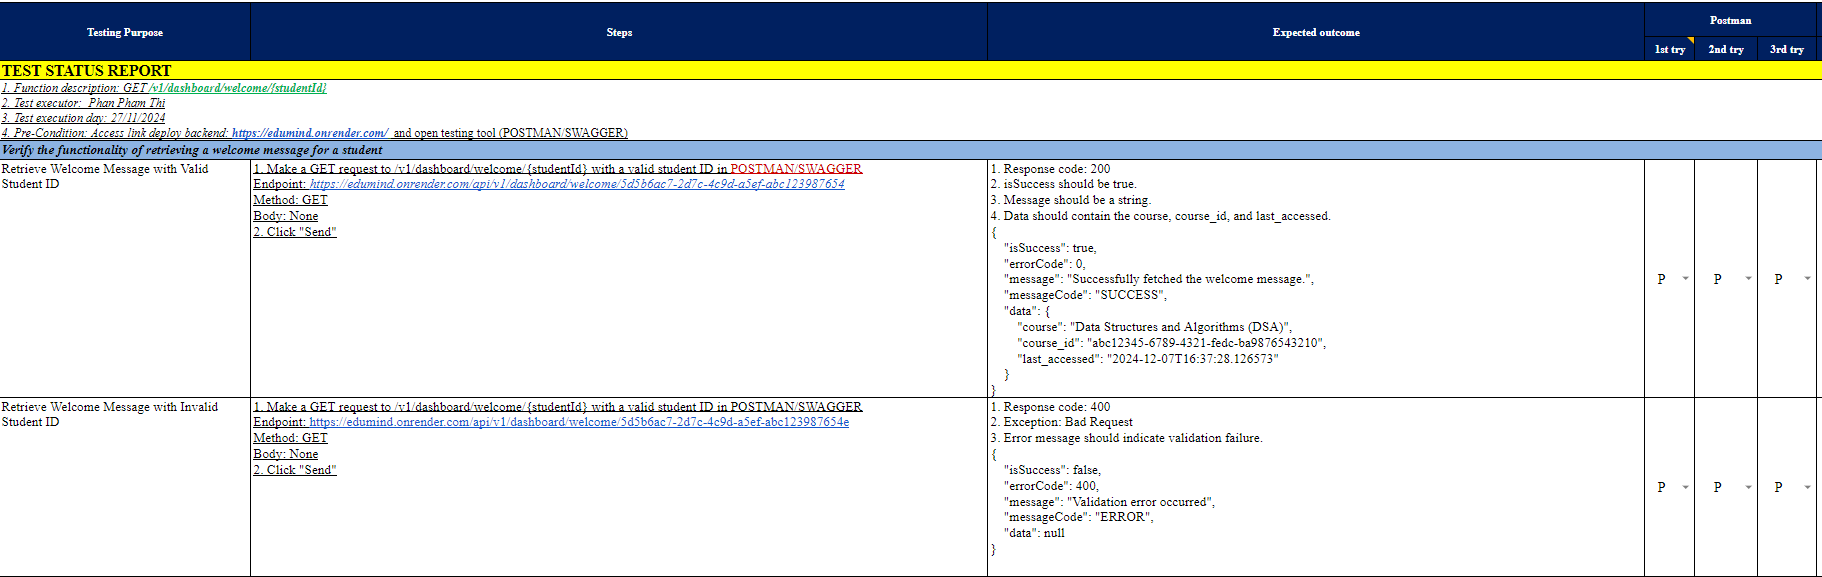
\includegraphics[width=0.8\textwidth]{Images/test/test_WC.png}
        \caption{Kiểm thử truy xuất các khóa học gần đây}
    \end{figure}
    Minh họa cách hệ thống truy xuất thông tin về các khóa học gần đây mà sinh viên đã tham gia hoặc có liên quan.
    \item \textbf{Get Activities API Testing}
    \begin{figure}[H]
        \centering
        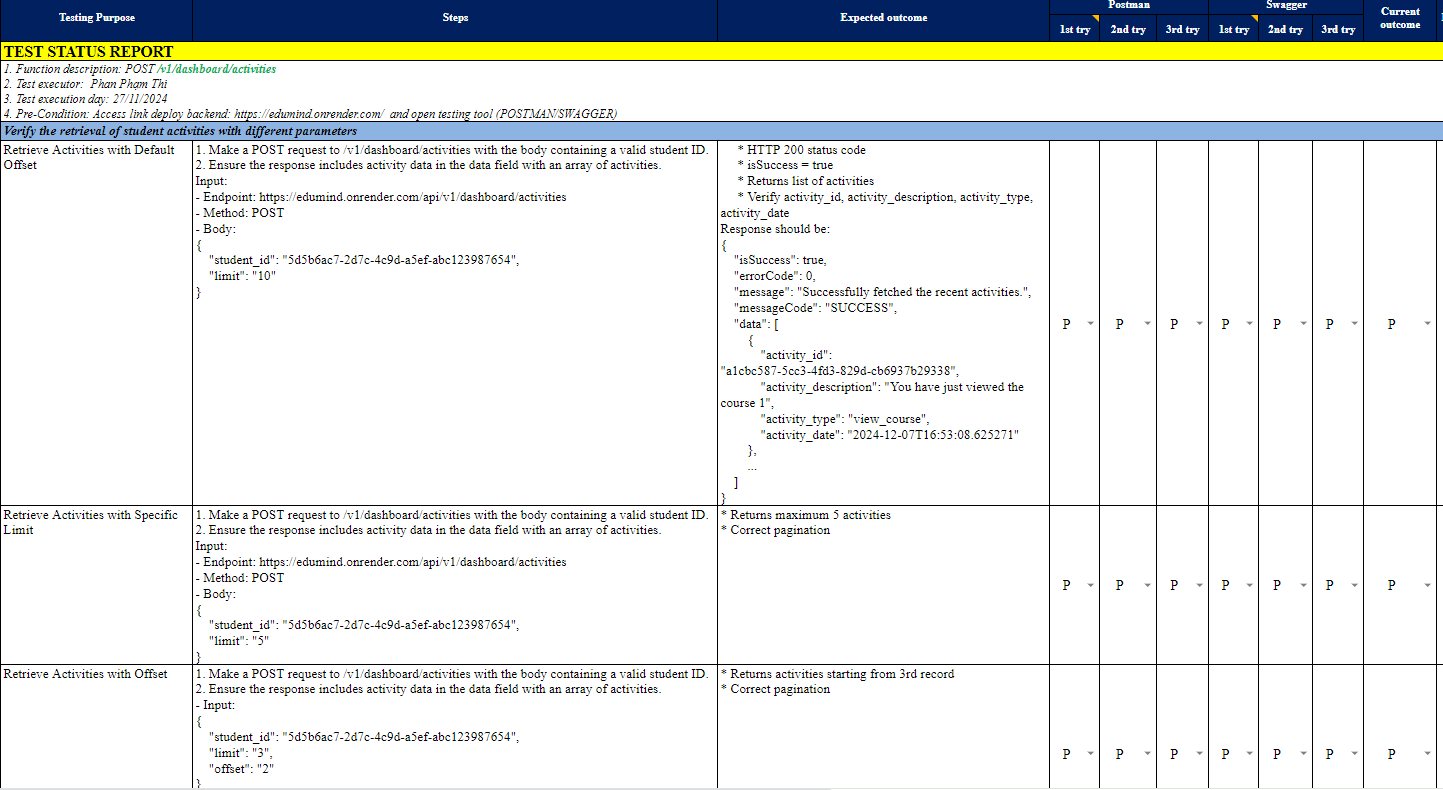
\includegraphics[width=0.8\textwidth]{Images/test/test_GA.png}
        \caption{Kiểm thử truy xuất các hoạt động gần đây}
    \end{figure}
    Hiển thị kết quả kiểm thử cho việc truy xuất các hoạt động gần đây của sinh viên trong hệ thống.
    \item \textbf{Courses List API Testing}
    \begin{figure}[H]
        \centering
        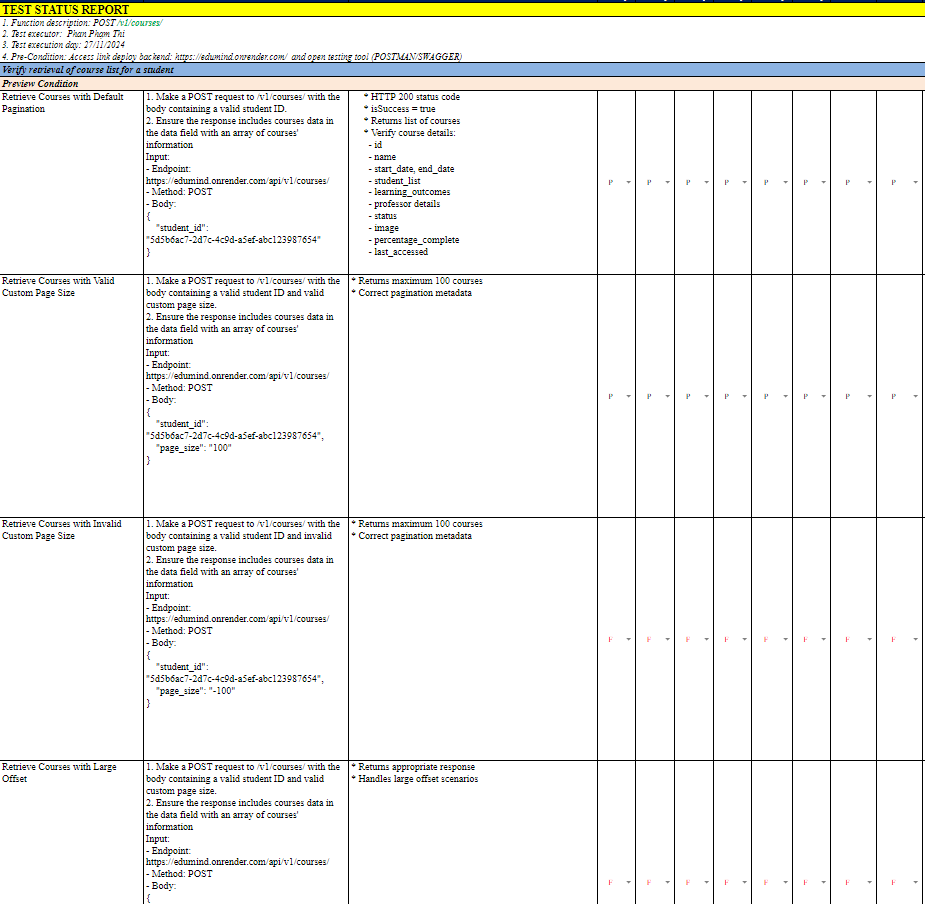
\includegraphics[width=0.8\textwidth]{Images/test/test_CL.png}
        \caption{Kiểm thử truy xuất danh sách khóa học của sinh viên}
    \end{figure}
    Thể hiện chi tiết kết quả khi lấy danh sách các khóa học mà sinh viên đã đăng ký hoặc tham gia.
    \item \textbf{Get Course for Student API Testing}
    \begin{figure}[H]
        \centering
        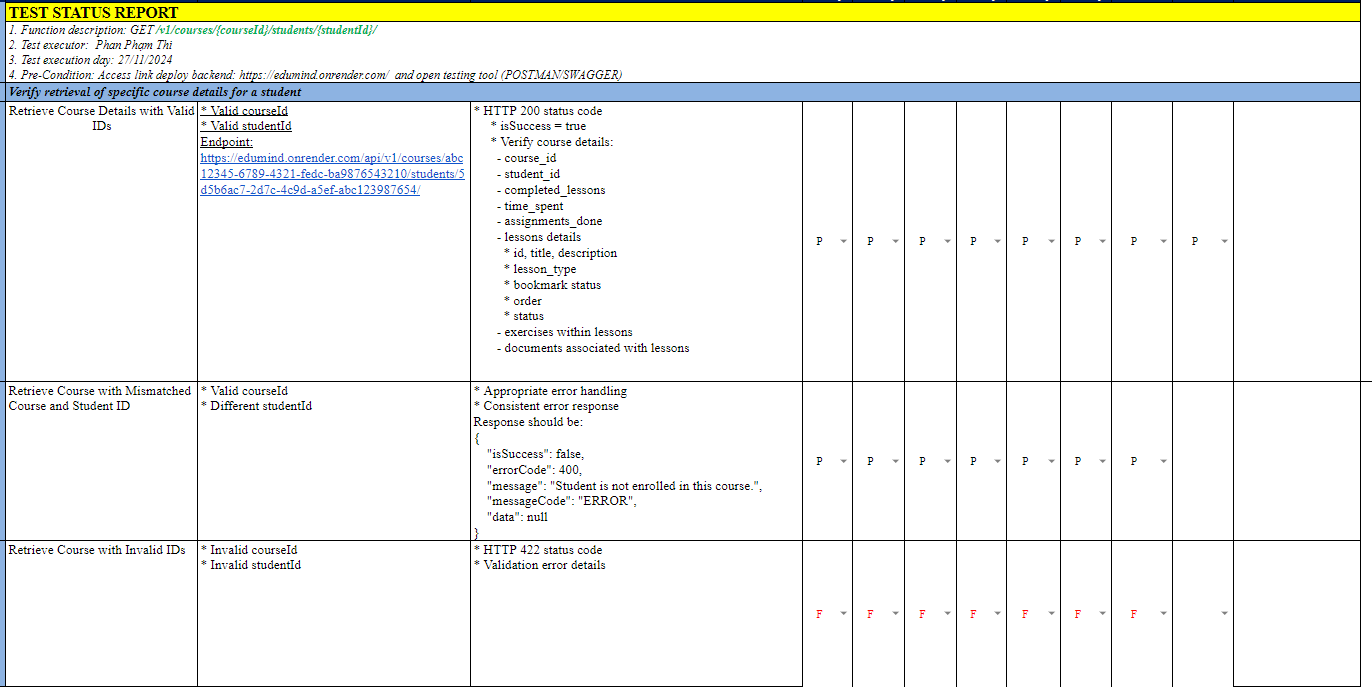
\includegraphics[width=0.8\textwidth]{Images/test/test_CD.png}
        \caption{Kiểm thử truy xuất chi tiết một khóa học}
    \end{figure}
    Kết quả trả về chi tiết thông tin của một khóa học cụ thể trong hệ thống.
    \item \textbf{Recommended Courses List API Testing}
    \begin{figure}[H]
        \centering
        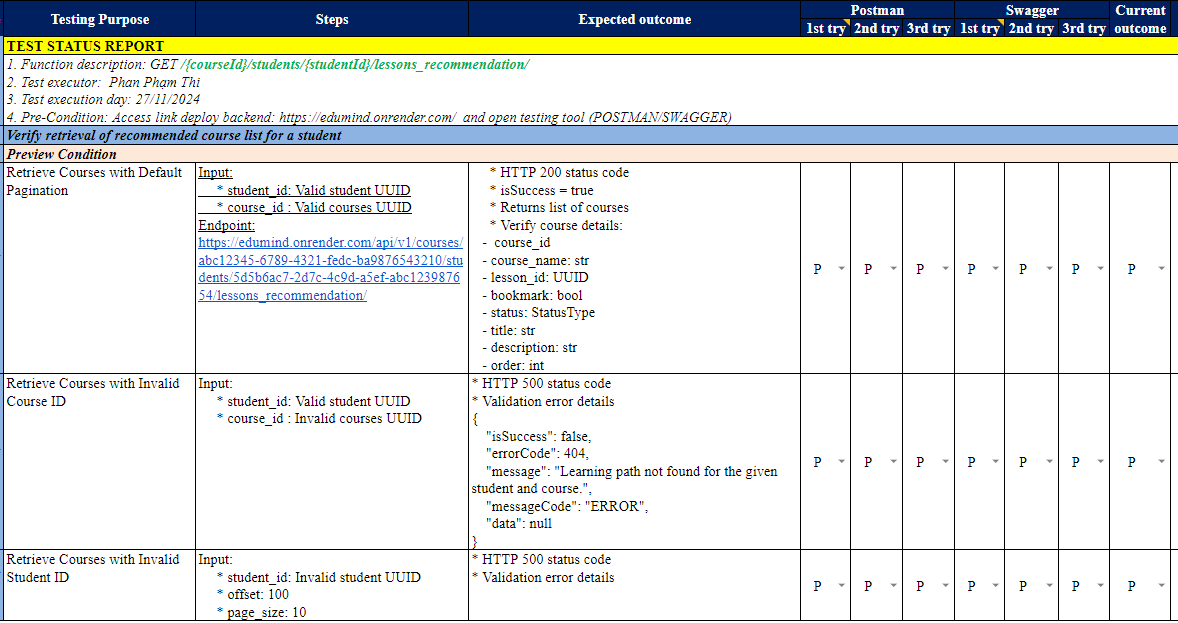
\includegraphics[width=0.8\textwidth]{Images/test/test_RCL.png}
        \caption{Kiểm thử truy xuất danh sách khóa học được đề xuất}
    \end{figure}
    Truy xuất danh sách các khóa học được hệ thống đề xuất dựa trên sở thích hoặc lịch sử học tập của sinh viên.
    \item \textbf{Add Activity API Testing}
    \begin{figure}[H]
        \centering
        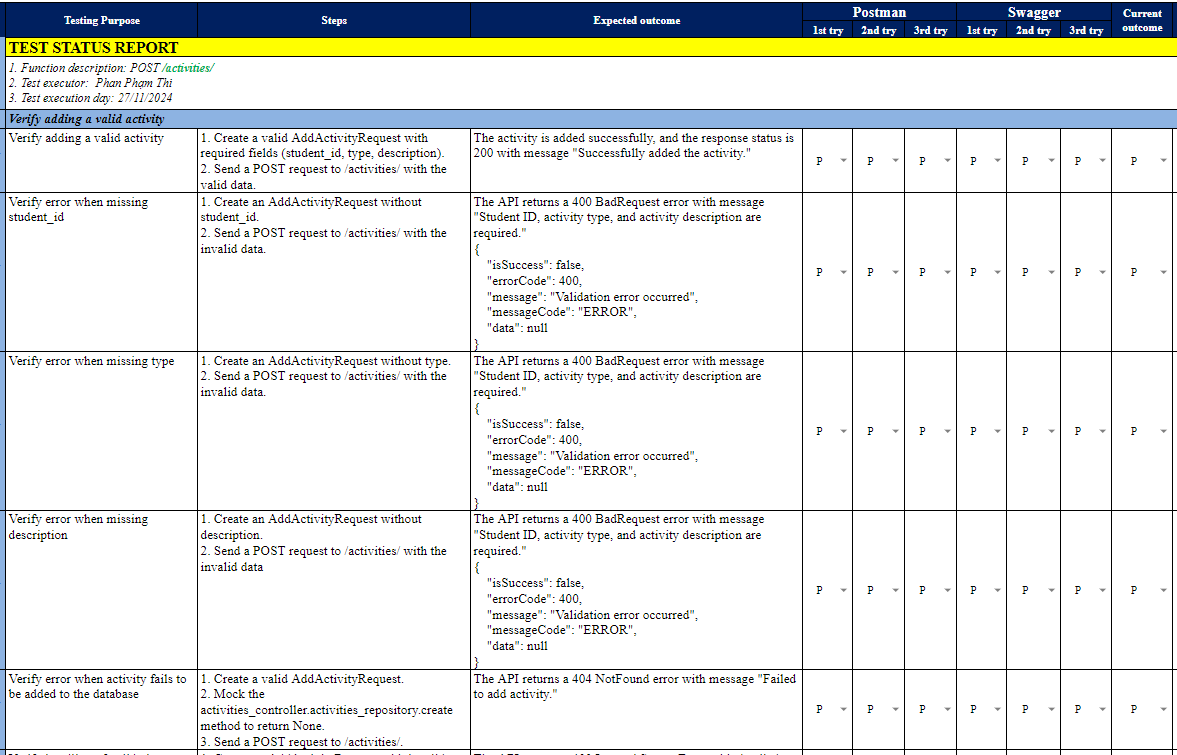
\includegraphics[width=0.8\textwidth]{Images/test/test_AA.png}
        \caption{Kiểm thử thêm hoạt động gần đây của sinh viên}
    \end{figure}
    Minh họa kiểm thử chức năng ghi nhận một hoạt động mới vào danh sách các hoạt động gần đây của sinh viên.
    \item \textbf{Recommend Lesson API Testing}
    \begin{figure}[H]
        \centering
        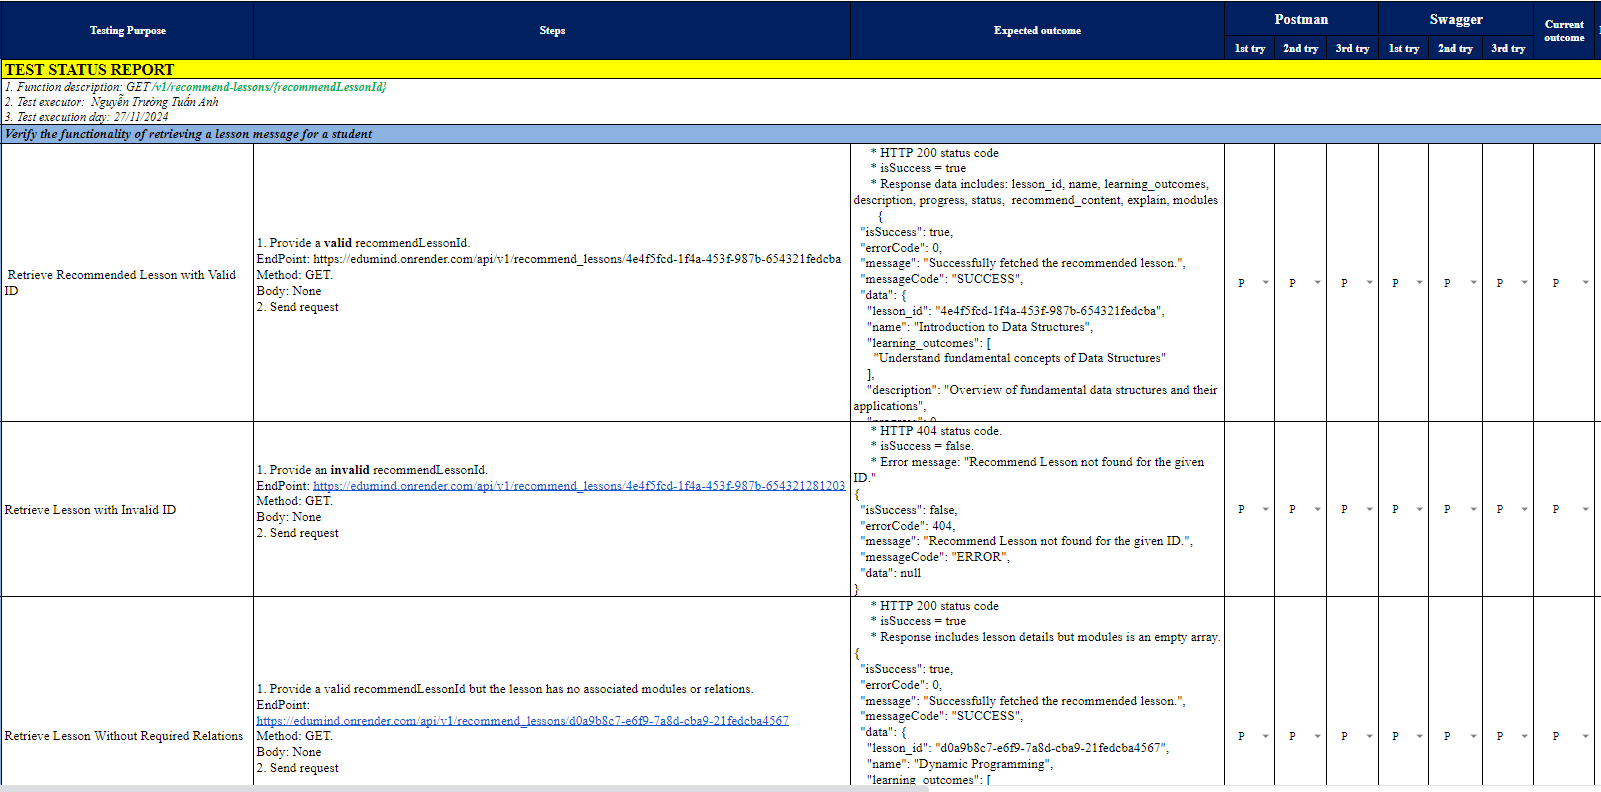
\includegraphics[width=0.8\textwidth]{Images/test/test_RL.png}
        \caption{Kiểm thử truy xuất chi tiết một lesson được đề xuất}
    \end{figure}
    Thể hiện kết quả kiểm thử khi truy xuất chi tiết về một bài học được hệ thống đề xuất.
    \item \textbf{Quizzes List API Testing}
    \begin{figure}[H]
        \centering
        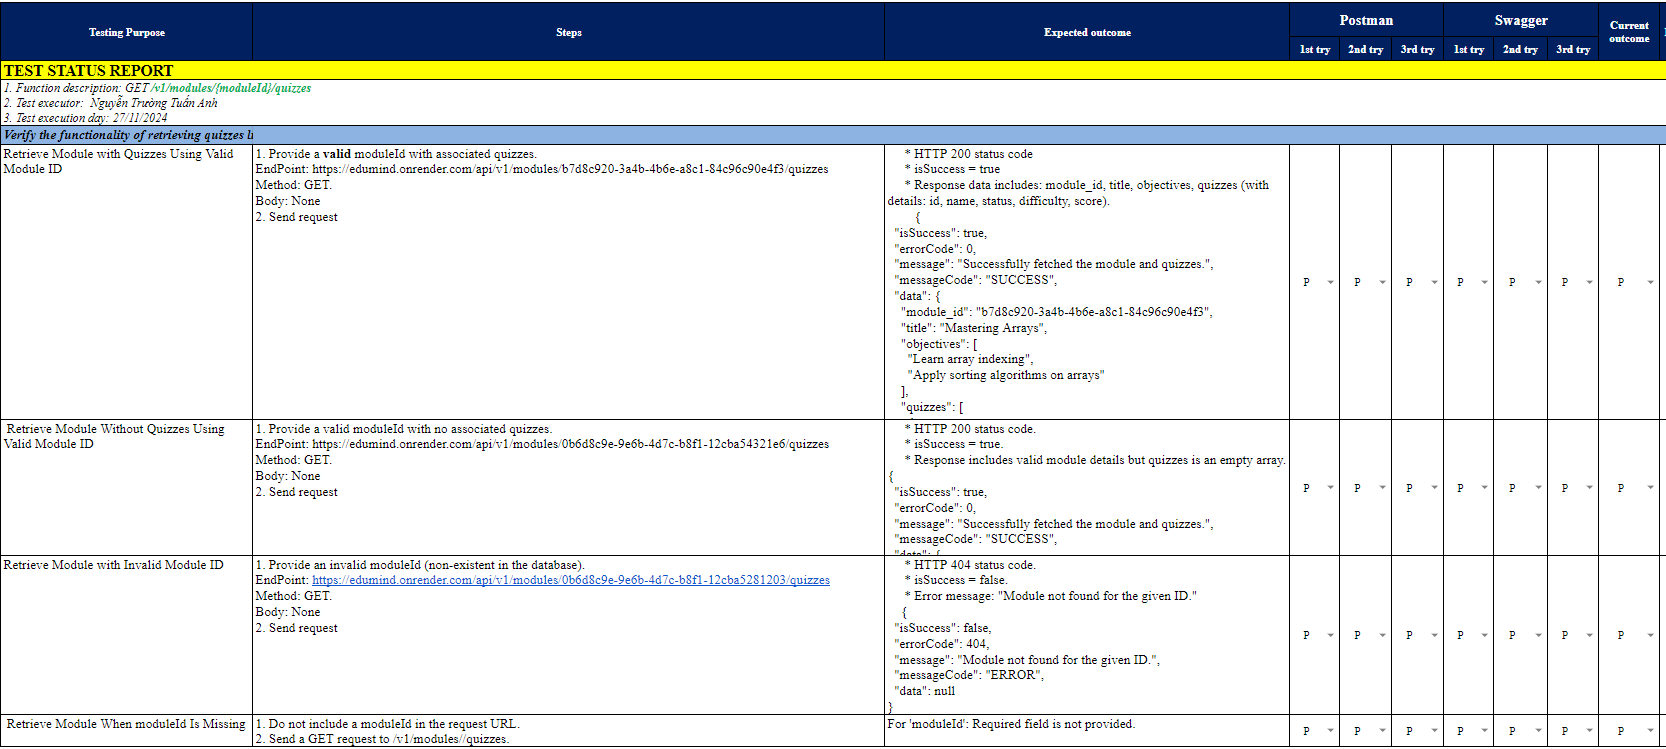
\includegraphics[width=0.8\textwidth]{Images/test/test_QL.png}
        \caption{Kiểm thử truy xuất danh sách bài tập quizzes từ module}
    \end{figure}
    Hiển thị kết quả kiểm thử danh sách bài tập dạng quiz từ một module cụ thể.
    \item \textbf{Quiz Detail API Testing}
    \begin{figure}[H]
        \centering
        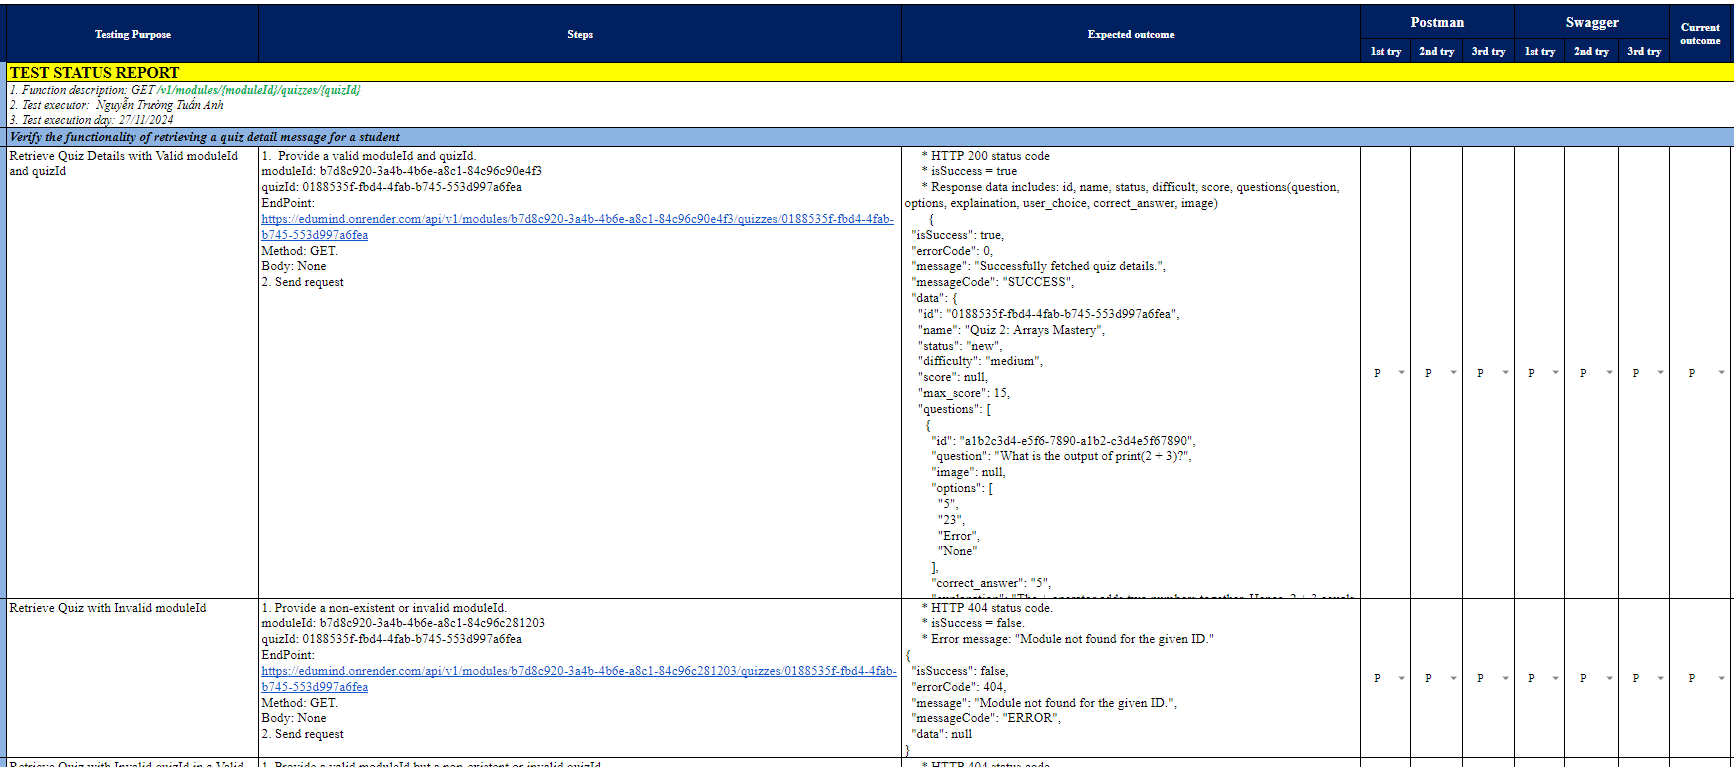
\includegraphics[width=0.8\textwidth]{Images/test/test_DQ.png}
        \caption{Kiểm thử truy xuất chi tiết một bài tập quiz}
    \end{figure}
    Kết quả kiểm thử truy xuất thông tin chi tiết về một bài tập quiz trong danh sách.
    \item \textbf{Clear Answer API Testing}
    \begin{figure}[H]
        \centering
        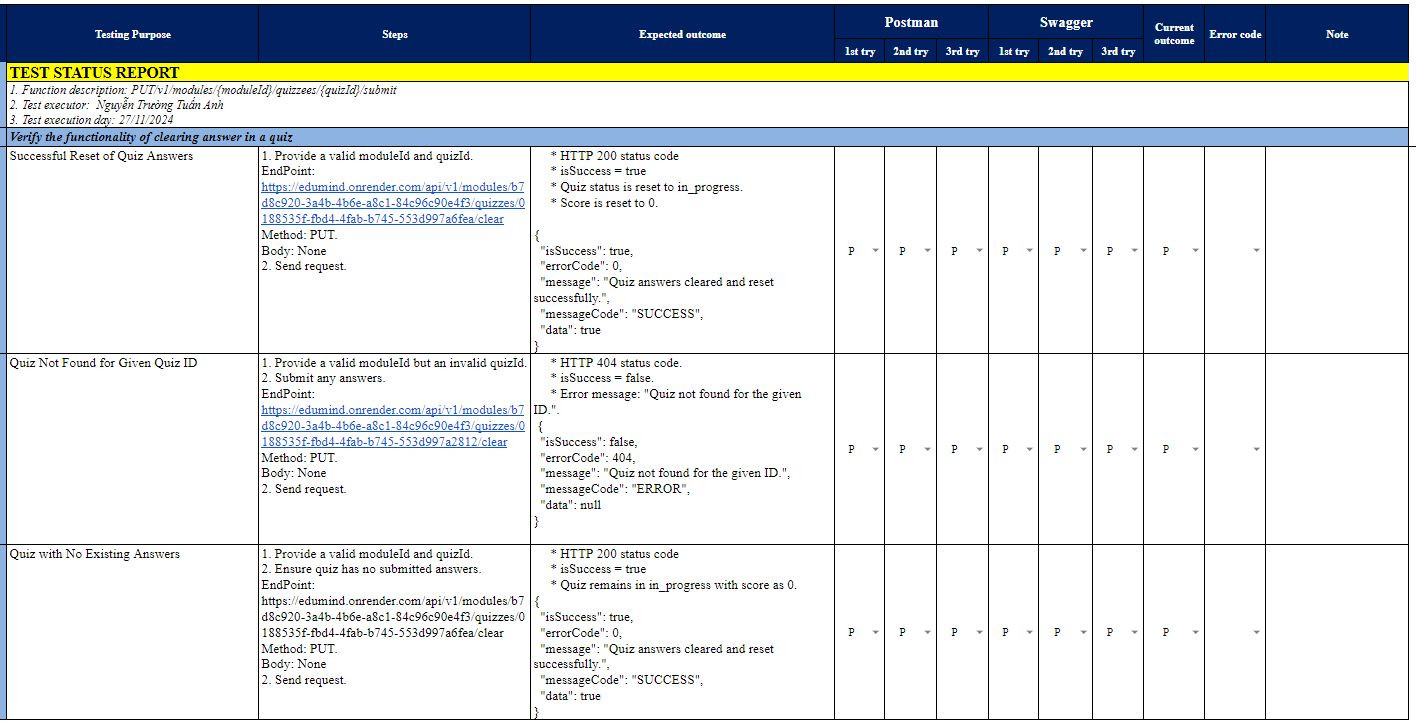
\includegraphics[width=0.8\textwidth]{Images/test/test_CA.png}
        \caption{Kiểm thử bắt đầu làm lại một bài tập quiz}
    \end{figure}
    Thể hiện kết quả thử nghiệm chức năng cho phép sinh viên bắt đầu làm lại một bài tập quiz đã làm trước đó.
    \item \textbf{Submit Answer API Testing}
    \begin{figure}[H]
        \centering
        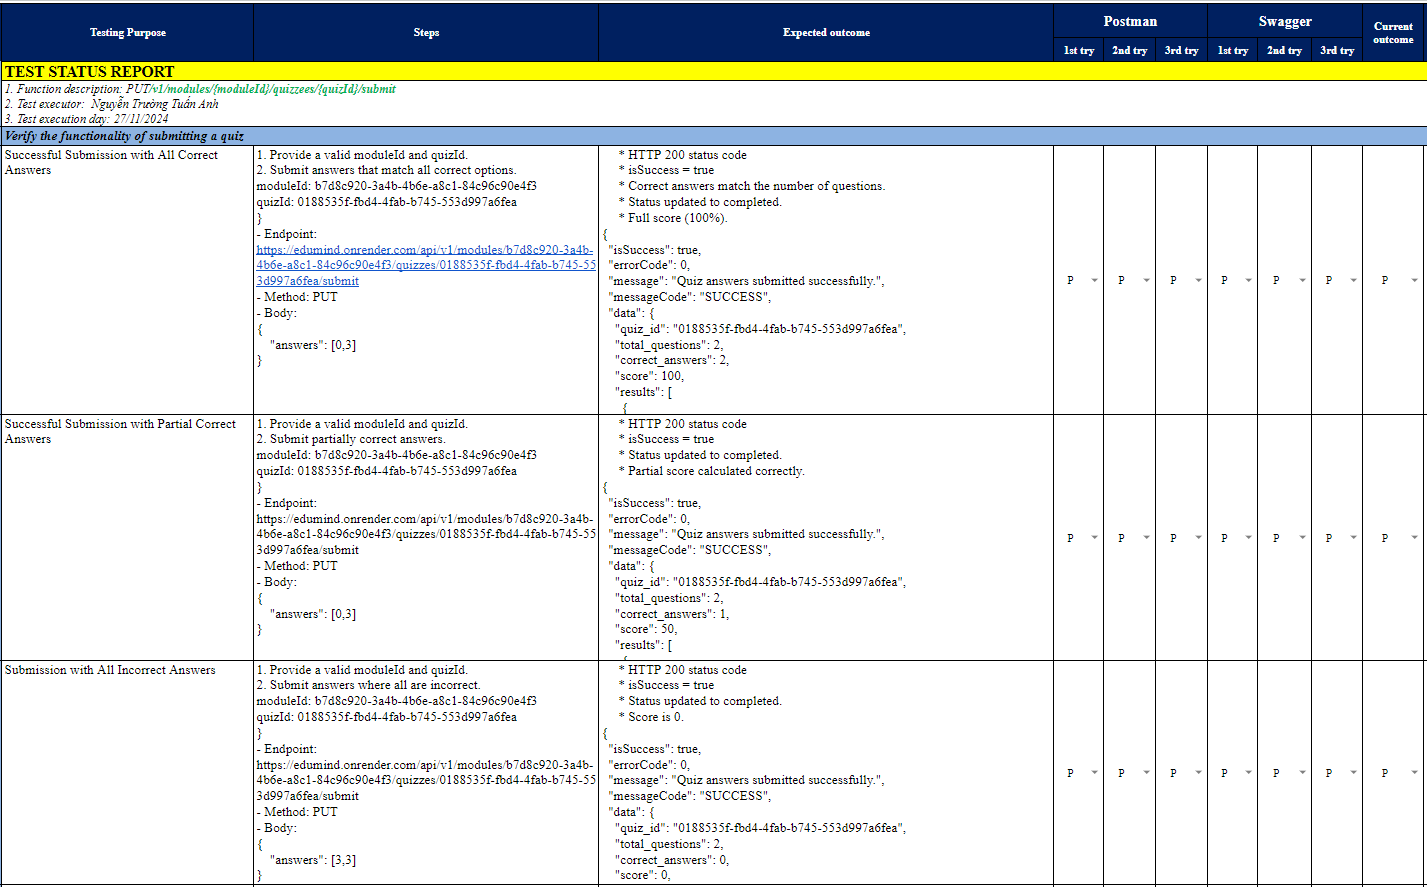
\includegraphics[width=0.8\textwidth]{Images/test/test_SA.png}
        \caption{Kiểm thử submit một bài tập quiz}
    \end{figure}
    Kiểm tra chức năng nộp bài làm cho một bài tập quiz thông qua hệ thống.
    \item \textbf{Document API Testing}
    \begin{figure}[H]
        \centering
        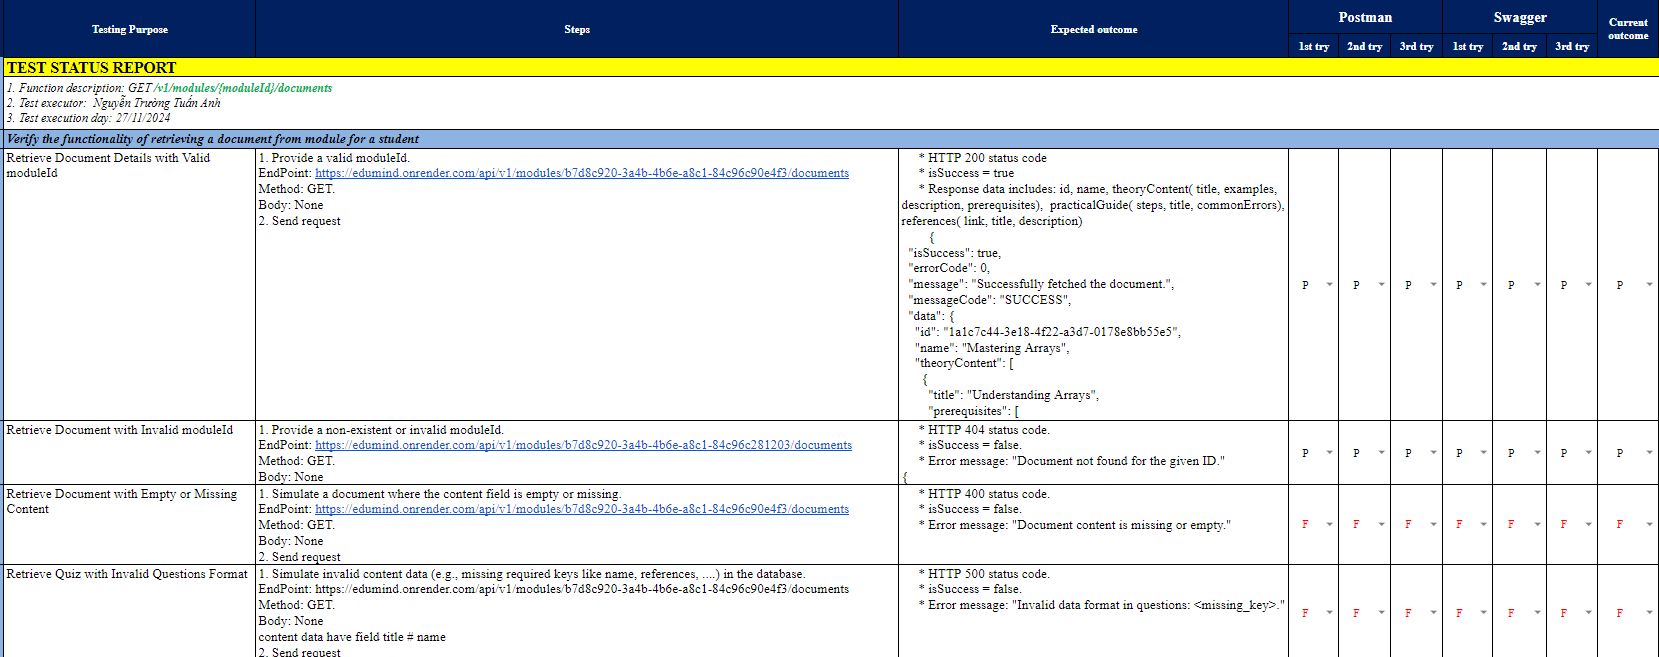
\includegraphics[width=0.8\textwidth]{Images/test/test_DO.png}
        \caption{Kiểm thử truy xuất document từ module}
    \end{figure}
    Minh họa việc truy xuất tệp tài liệu từ một module khóa học.
\end{itemize}
\subsubsubsection{Kết quả tổng hợp của các testcase}
\begin{figure}[H]
    \centering
    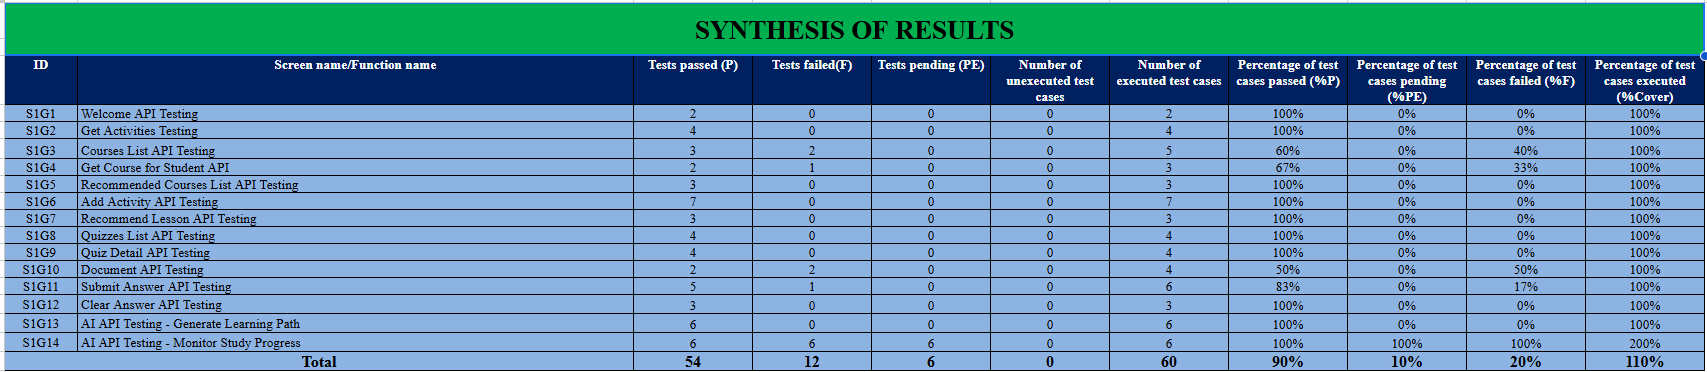
\includegraphics[width=0.8\textwidth]{Images/test/synthesisResults.png}
    \caption{Kết quả tổng hợp của các testcase}
\end{figure}
\begin{itemize}
    \item Kết quả tổng quan:
    \begin{itemize}
        \item \textbf{Số lượng test case đã thực thi:} Toàn bộ 48 test case đã được thực thi, đạt tỷ lệ bao phủ kiểm thử là 100\%.
        \item \textbf{Số lượng test case đã vượt qua:} Có 42 test case thành công, chiếm 88\% tổng số test case.
        \item \textbf{Số lượng test case thất bại:} Có 6 test case thất bại, chiếm 13\% tổng số test case.
        \item \textbf{Số lượng test case đang chờ xử lý:} Không có test case nào đang chờ xử lý (0\%).
    \end{itemize}
    \item Phân tích chi tiết theo từng chức năng
    \begin{itemize}
        \item \textbf{Welcome API Testing, Get Activities Testing, Recommended Courses List API Testing, Add Activity API Testing, Recommend Lesson API Testing, Quizzes List API Testing, Quiz Detail API Testing, Clear Answer API Testing:} 
        Các chức năng này đều đạt tỷ lệ thành công 100\%, không có lỗi xảy ra trong quá trình kiểm thử.
        
        \item \textbf{Courses List API Testing:} Tỷ lệ thành công đạt 60\% với 3 test case vượt qua và 2 test case thất bại.
        
        \item \textbf{Get Course for Student API:} Tỷ lệ thành công đạt 67\%, với 2 test case vượt qua và 1 test case thất bại.
        
        \item \textbf{Document API Testing:} Có tỷ lệ thành công thấp nhất (50\%), với 2 test case vượt qua và 2 test case thất bại.
        
        \item \textbf{Submit Answer API Testing:} Đạt tỷ lệ thành công 83\%, với 5 test case vượt qua và 1 test case thất bại.
    \end{itemize}
\end{itemize}